\documentclass{article}
\usepackage{graphicx} % Required for inserting images

\title{Assignment 1}
\author{Jinyao DeSandies}
\date{August 2025}

\begin{document}

\maketitle

\section{Some Notes}
\emph{   emph is emphasis}
\textit{ textit is italics}
\textbf{ textbf is bold font}
% are comments
\section{Name, Pronouns}
My name is Jinyao\ref{fig:me}. I go by He/Him/His. I can be very talkative at times. 
\begin{figure}
    \centering
    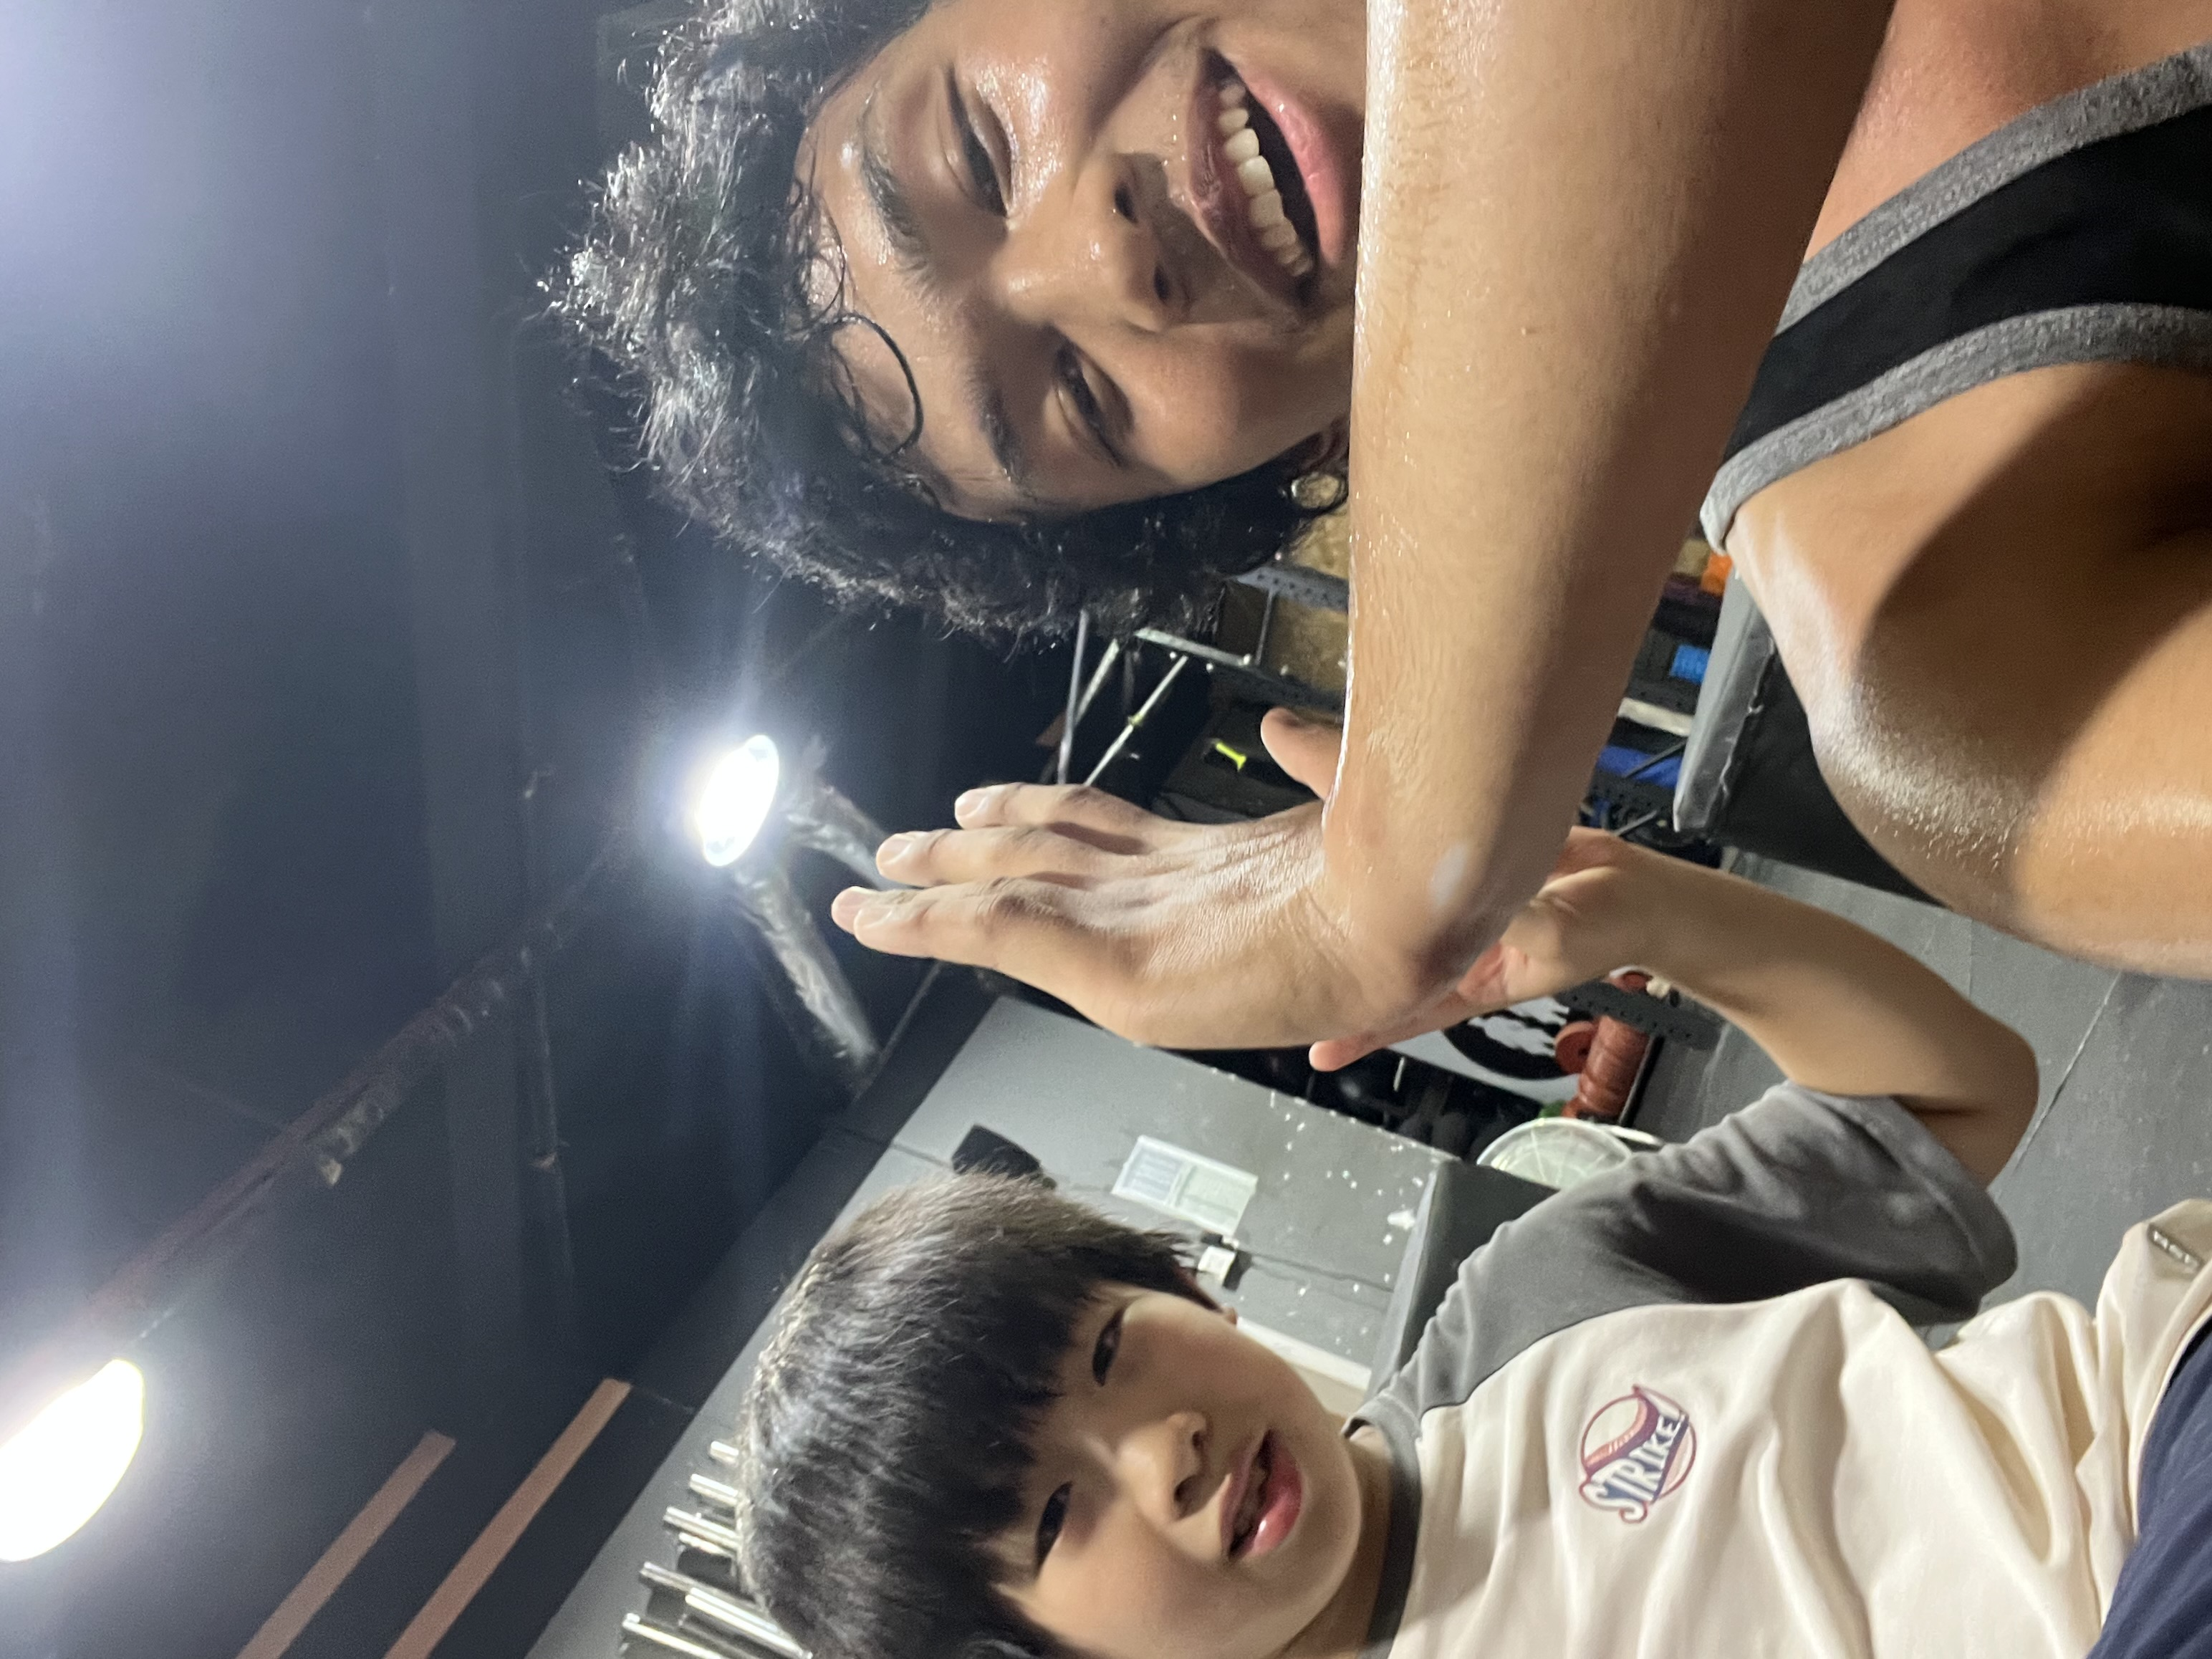
\includegraphics[width=0.5\linewidth]{IMG_3908.jpeg}
    \caption{Caption}
    \label{fig:me}
\end{figure}


Please feel free to interrupt me when I talk too much. It's likely better for us dynamically

\section{Where I'm From}
I am from \emph{Guangzhou, China}\ref{fig:Zhujiang Newtown}. It is in the south of China. It is a very hot place\ref{weather}. I went to ISA Science city
\subsection{Guangzhou Temperature}
\begin{tabular}{c c| c| c| c| c| c| c| c}
         Day &1 & 2&3&4&5&6&7&8 \\
        Highest&97&96&91&91&95&93&93&94 \\
        Lowest& 79&80&79&78&80&78&79&78
        \label{weather}
    \end{tabular}
\begin{figure}
    \centering
    \includegraphics[width=0.5\linewidth]{IMG_1973.jpeg}
    \caption{A skyline of China (there are many more)}
    \label{fig:Zhujiang Newtown}
\end{figure}
\section{Prior Programming Experience}
I have various forms of programming experience, including \ref{item}
\begin{itemize}
    \item Python
    \item HTML
    \item CSS
    \item a little bit of R
    \item now LaTeX
    \label{item}
\end{itemize}

\begin{center}
I am not in CSCI 050
\end{center}
\section{what do I want to study}
I want to study Computer Science. My long term goal is to become rich so I can make a real, positive impact in this capitalist society.

\section{Free Time}
\begin{figure}
    \centering
    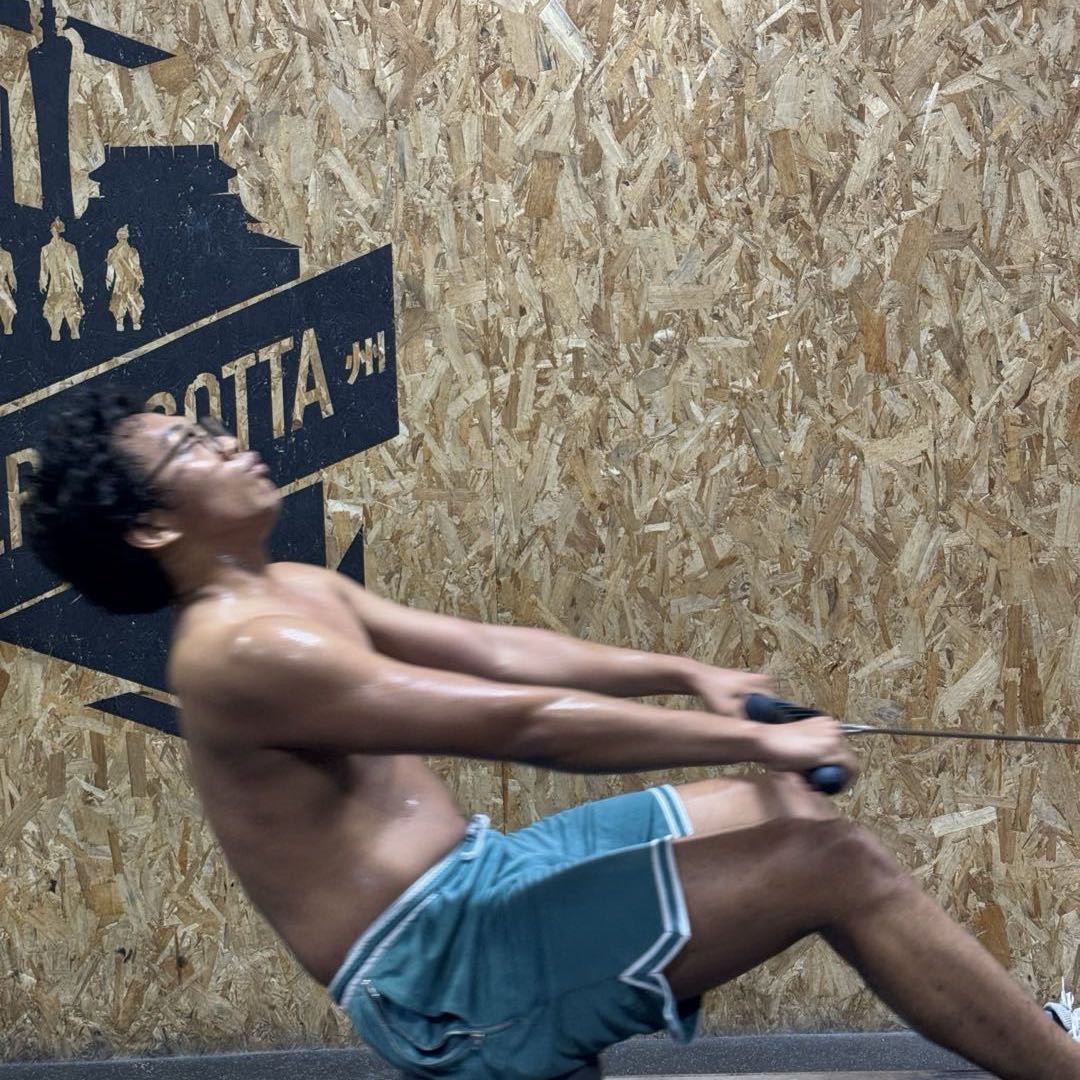
\includegraphics[width=0.5\linewidth]{IMG_3086.jpeg}
    \caption{Rowing}
    \label{fig:weightlift}
\end{figure}
\begin{figure}
    \centering
    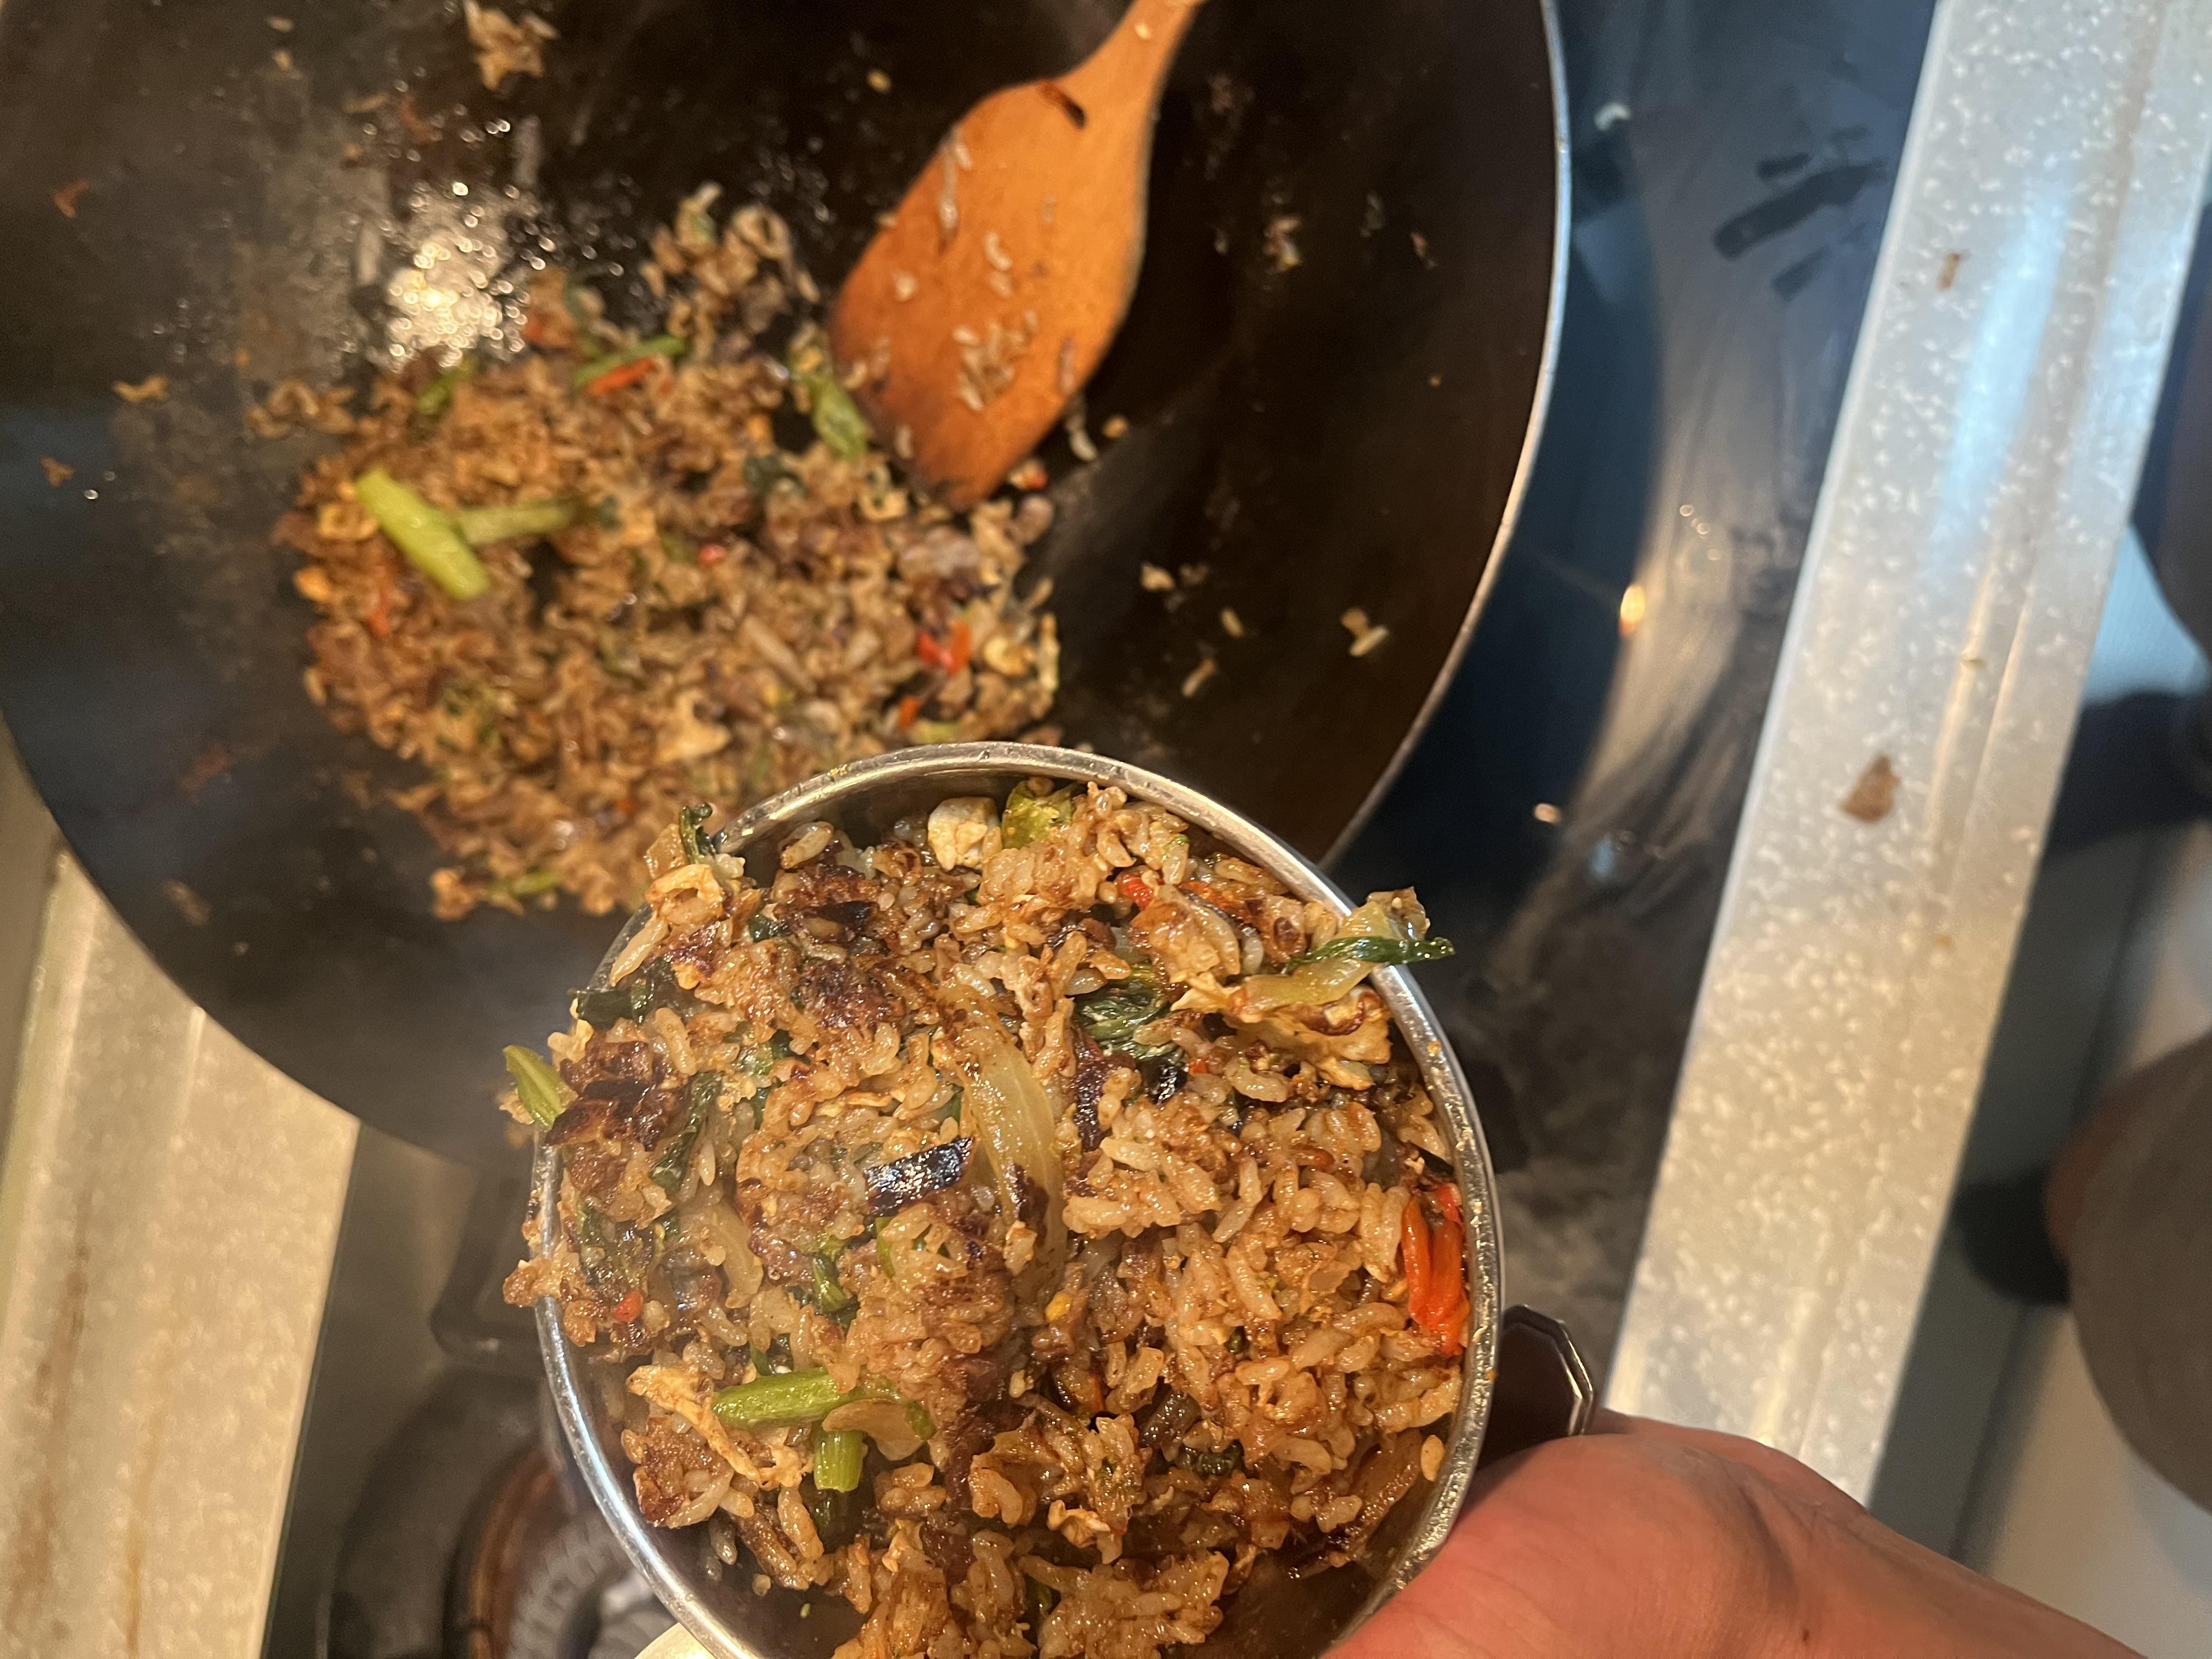
\includegraphics[width=0.5\linewidth]{IMG_2491.jpeg}
    \caption{Fried Rice}
    \label{fig:cooking}
\end{figure}
I like to Weightlift\ref{fig:weightlift}, Cook\ref{fig:cooking}, etc.
\newpage
\begin{center}
    

\section{What I value the most}
Love- friends, family, romantically
\section{Aspects to the course
}
\subsection{Im looking forward to}
Learning deep computer science courses
\subsection{I'm nervous that}
I already did most of the stuff in the syllabus
\subsection{I found interesting}
the turning machine designed to make advanced calculations seemed really cool. I would love to learn more about it at some point.
\subsection{what else I want to know}
Any jobs for me as a Freshman?
\end{center}
\end{document}

- What name would you like to be called? Do you want to tell us your personal pronoun? Isthere anything else I should know?
- Where are you from? Where did you go to high school?
- Do you have any prior programming experience?
- Are you concurrently enrolled in CSCI050?
- What are your academic interests and/or planned major? Do you have a long-term goal or
dream job in mind for the future?
- What do you enjoy doing in your free time?
- What do you value the most?
- Which aspects of this course are you most looking forward to?
- Which aspects of this course are you most nervous about?
- What stood out to you about what we covered this week, either on the history or ethics of
computer science?
- Is there anything else you’d like us to know?

